\documentclass[a4paper,11pt]{article}

\usepackage[utf8]{inputenc}	
\usepackage[T1]{fontenc}
\usepackage{lmodern}
\usepackage{times}
\usepackage[margin=2cm]{geometry}
\usepackage{amsmath}
\usepackage{mathtools}
\usepackage{graphicx}
\usepackage{multirow}
\usepackage{blindtext}
\usepackage{hyperref}

\usepackage{pgfplotstable} 
\usepackage{booktabs}

\graphicspath{ {./images/} }

\usepackage[czech]{babel}
\usepackage{graphicx}
\usepackage{amsmath}
\usepackage{xspace}
\usepackage{url}
\usepackage{indentfirst}
\usepackage{subcaption}
\usepackage{caption}
\usepackage{tabularx}
\usepackage{rotating}
\usepackage{tikz}
\usepackage[labelformat=parens,labelsep=quad,skip=3pt]{caption}

\usepackage{color}  
\usepackage{listings}

\definecolor{codegreen}{rgb}{0,0.6,0}
\definecolor{codegray}{rgb}{0.5,0.5,0.5}
\definecolor{codepurple}{rgb}{0.58,0,0.82}
\definecolor{backcolour}{rgb}{0.95,0.95,0.92}

\lstdefinestyle{mystyle}{
    backgroundcolor=\color{backcolour},   
    commentstyle=\color{codegreen},
    keywordstyle=\color{magenta},
    numberstyle=\tiny\color{codegray},
    stringstyle=\color{codepurple},
    basicstyle=\ttfamily\footnotesize\centering,        
    breaklines=true,                 
    captionpos=b,                                  
    numbers=left,                    
    numbersep=5pt,                  
    showspaces=false,              
    showstringspaces=false,
    showtabs=false,                  
    tabsize=2
}

\lstset{style=mystyle}


\widowpenalty 10000 \clubpenalty 10000 \displaywidowpenalty 10000
\setcounter{topnumber}{3}	  
\setcounter{bottomnumber}{3}	 
\setcounter{totalnumber}{6}	  
\renewcommand\topfraction{0.9}	 
\renewcommand\bottomfraction{0.9} 
\renewcommand\textfraction{0.1}	  
\intextsep=8mm \textfloatsep=8mm 

\renewcommand{\thesection}{\arabic{section}.}
\renewcommand{\thesubsection}{\thesection\arabic{subsection}.}
\makeatletter \def\@seccntformat#1{\csname the#1\endcsname\hspace{1ex}} \makeatother


\begin{document}

\hline
\begin{center}
\bigskip
\huge Určení polohy Barnardovy hvězdy na nebeské sféře
\vspace{0.5cm}
\par \large F4191: Praktikum z astronomie 2
\par \large Artem Gorodilov
\vspace{0.5cm}
\par \large 30. ~října 2024
\bigskip
\end{center}
\hline
\bigskip


\vskip10pt
    \begin{minipage}[t]{0.5\textwidth} 
        \section{Abstrakt}    
            V této práci jsme určili přesnou polohu hvězdy Barnadra k datu 01.05.2024 02:06 (UT). Pozorování bylo provedeno na Vyškovské hvězdárně (17.02236954$^o$, 49.28377745$^o$) ve filtru Halfa, expoziční doba 30 s.
            \par Výpočty byly provedeny pomocí skriptu v Pythonu\textsuperscript{\cite{github}}.

        \section{Zpracování dat}
            \subsection{Popis paipelinu}    
                Jako vstupní data skript použije tabulku \texttt{"data/positions.csv"}, jejíž data jsou ve formátu: 
                \vspace{5pt}
                \par ra,dec,X,Y
                \par "17:57:24.446","+04:36:08.11",1292.5,1651.1667
                \par ...
                \vspace{10pt}
                \par kde ra,dec jsou souřadnice hvězd převzaté z databáze Aladin\textsuperscript{\cite{aladin}} a X,Y jsou souřadnice stejných hvězd v osách Image X a Image Y.

\begin{lstlisting}[language=Python]
# Importing data
data = pd.read_csv('data/positions.csv')
\end{lstlisting}

                \par Dále načteme náš .fits snimek pomocí knihovny \texttt{astropy} a určíme jeho střed v pixelech. V naší práci jsme analyzovali snimek barnard\_2024-05-01\_02-06-51\_Halpha\_0310.fits.

\begin{lstlisting}[language=Python]
# Loading images
image_path = glob.glob(f"data/*.fits")
images = [fits.getdata(image_path) for image_path in image_path]

# Find the center of the image
x_center, y_center = (images[0].shape[1] // 2, images[0].shape[0] // 2)
\end{lstlisting}

                Střed snimku (neboli střed CCD čipu):
                \begin{center}
                    x$_{center}$ = 1028 px, y$_{center}$ = 1031 px
                \end{center}

    \end{minipage}
    \hspace{10pt}
    \begin{minipage}[t]{0.5\textwidth} 
                Pak jsme transformovali souřadný systém tak, že počátek (0,0) je v bodě (x$_{center}$, y$_{center}$):

\begin{lstlisting}[language=Python]
# Convert coordinate system to have (0,0) at (x_center, y_center)
data['X'] = data['X'] - x_center
data['Y'] = data['Y'] - y_center 
\end{lstlisting}

                \par Dále jsme převedli Ra a Dec z \texttt{positions.csv} na desetinné stupně pomocí \texttt{ra\_to\_decimal()} a \texttt{dec\_to\_decimal()}.

\begin{lstlisting}[language=Python]
# Convert RA and Dec to decimal degrees
data['ra'] = data['ra'].apply(ra_to_decimal)
data['dec'] = data['dec'].apply(dec_to_decimal)
\end{lstlisting}

                \par Protože byl náš obrázek otočen vzhledem k původním souřadnicím Ra a Dec a posunut podél příslušných os, musíme vypočítat parametry těchto transformací. To jsme provedli pomocí afinní transformace zobrazení:

                \begin{center}
                    \begin{equation}
                        \begin{bmatrix} X$_{trans}$ \\ Y$_{trans}$ \end{bmatrix} = \begin{bmatrix} a & b \\ b & -a \end{bmatrix} \begin{bmatrix} X \\ Y \end{bmatrix} + \begin{bmatrix} c \\ d \end{bmatrix}
                    \end{equation}
                \end{center}
                
                \begin{center}
                    \begin{equation}
                        X_{trans} = aX + bY + c 
                    \end{equation}
                    \begin{equation}
                        Y_{trans} = bX - aY + d
                    \end{equation}
                \end{center}

                \par kde jsme pomocí knihovny \texttt{scipy} a metody nejmenších čtverců \texttt{least\_squares} zjistili koeficienty a a b (koeficienty rotace), c a d (koeficienty posunu).
                
                \par Dále jsme určili směrodatné odchylky pomocí funkce \texttt{residuals()} a jacobianu transformace, ze které jsme pak získali kovarianční matici, jejíž kořeny diagonálních prvků jsou směrodatné odchylky parametrů a,b,c,d. 

                \begin{center}
                    $p=[a,b,c,d]^T$ - koeficienty transformace
                    \vspace{5pt}
                    \par Cov(p) = $\sigma^2$ (J$^T$J)$^{-1}$ - kovarianční matice
                    \vspace{5pt}
                    \par $\sigma_{p}$ = $\sqrt{diag(Cov(p))}$ - směrodatné odchylky
                \end{center}
    \end{minipage}
\newpage
    \begin{minipage}[t]{0.5\textwidth} 
                \par kde $\sigma^2$ je střední hodnota kvadrátu reziduí, J je jakobian transformace.
                \par Pro výpočet úhlu otočení kamery $\theta$ vzhledem k souřadnicím použijeme vzorec: 
                \begin{equation}
                    \theta = \arctan{\frac{b}{a}}
                \end{equation}

                \par Nakonec můžeme pomocí funkce \texttt{transform\_coordinates()} a zjištěných parametrů a,b,c,d vypočítat skutečné Ra a Dec pro libovolné vybrané objekty se souřadnicemi X a Y.

                \par Zorné pole jsme vypočítali tak, že jsme zjistili krajní hodnoty Ra, Dec pro osy X a Y a jednu od druhé odečetli. 
                \par Rozlišení kamery jsme určili jako: 
                \begin{equation}
                    R = \sqrt{a^2 + b^2} \cdot 3600
                \end{equation}

\begin{lstlisting}[language=Python]
# Calculate FOV
ra_min_comb, dec_min_comb = transform_coordinates(-x_center, -y_center, params_comb)
ra_max_comb, dec_max_comb = transform_coordinates(x_center, y_center, params_comb)

fov_ra = (ra_min_comb - ra_max_comb) * 3600
fov_dec = (dec_min_comb - dec_max_comb) * 3600

# Calculate resolution
resolution = sqrt(params_comb[0]**2 + params_comb[1]**2) * 3600
\end{lstlisting}

\par Při znalosti fyzické velikosti pixelů čipu CCD (S = 7.4x7.4 $\mu$m$^2$) a rozlišení kamery jsme byli schopni určit ohniskovou vzdálenost dalekohledu pomocí funkce \texttt{calculate\_focal\_length()}.
\begin{equation}
    f = \frac{S}{R} \cdot 206265
\end{equation}
kde S je velikost pixelu, R je rozlišení kamery. 

        \section{Výsledky}  
                Pro určení transformačních parametrů jsme vybrali 21 hvězd určením jejich polohy na snímku (X,Y) a jejich souřadnic z Aladinu (Ra, Dec). Údaje jsou uvedeny v tabulce (1) a na obrázku (\ref{fig:barnard_sky}).

                \par Jako instrumentální chybu jsme použili tyto hodnoty:
                \begin{center}
                    $\sigma_{x,y}$ = 0.5 px, $\sigma_{ra,dec}$ = 0.1 arcsec
                \end{center}

                \par Určili jsme transformační parametry a,b,c,d: 

                \begin{center}
                    a = 5.37(1)$\cdot$10$^{-5}$ [deg/px], b = -2.128(1)$\cdot$10$^{4}$ [deg/px],
                    \vspace{5pt}
                    \par c = 269.46954(7) [deg], d = 4.69246(7) [deg]
                \end{center}
    \end{minipage}
    \hspace{10pt}
    \begin{minipage}[t]{0.5\textwidth}
                Z toho jsme určili úhel otočení $\theta$:

                \begin{center}
                    $\theta$ = -75.84(3) [deg]
                \end{center}

                \par Poté jsme určili souřadnice středu čipu:

                \begin{center}
                    X$_{center}$ = 1028 px, Y$_{center}$ = 1031 px
                    \vspace{5pt}
                    \par Ra$_{center}$ = 17:57:52.69(3) [h], 
                    \par Dec$_{center}$ = +04:41:32.9(5) [deg]
                \end{center}
                        
                \par Poté jsme určili souřadnice Barnardovy hvězdy: 

                \begin{center}
                    X$_{Barnard}$ = 687.7441 px, Y$_{Barnard}$ = 1051.81917 px
                    \vspace{5pt}
                    \par Ra$_{Barnard}$ = 17:57:47.24(3) [h], 
                    \par Dec$_{Barnard}$ = +04:45:49.6(5) [deg]
                \end{center}
                
                \par Poté jsme vypočítali zorné pole kamery:

                \begin{center}
                    FOV$_{ra}$ = 1183(1) [arcsec], FOV$_{dec}$ = 1974(1) [arcsec]
                \end{center}
                
                \par A také rozlišení kamery: 

                \begin{center}
                    R = 0.7902(4) [arcsec/px]
                \end{center}
                
                \par Velikost čipu je 2056x2062.
                
                \par Ohniskovou vzdálenost dalekohledu jsme určili jako:

                \begin{center}
                    \par f = 1.9316(9) [m]
                \end{center}
                
                \par Pro kontrolu jsme vynesli do grafu hodnoty Ra a Dec, které jsme získali, a hodnoty získané z Aladinu. Výsledky jsou znázorněny na obrázku (\ref{fig:barnard_radec}).
                \par K ověření správné identifikace Barnardovy hvězdy jsme použili data Gaia DR3 a práci (Buchheim+)\textsuperscript{\cite{Buchheim}}.
                \par Jak je vidět, hvězda má vysoký vlastní pohyb, který jsme také vypočítali:
                \begin{center}
                    $\mu_{ra}$ = (-752$\pm$30) [mas/yr], 
                    \par $\mu_{dec}$ = (10427$\pm$30) [mas/yr]
                \end{center}
           
        \section{Závěr}
                Jak je patrné z obrázku (2), parametry transformace byly určeny správně. Totéž lze říci o úhlu otočení. Hodnoty zorného pole a rozlišení kamery se zdají být důvěryhodné, ale bylo by dobré je porovnat se skutečnými údaji. Na základě zjištěných rychlostí vlastního pohybu hvězdy a jejich porovnání s údaji z literatury \textsuperscript{\cite{Buchheim}}, můžeme říci, že jsme správně identifikovali Barnardovu hvězdu.

                \begin{center}
                    $\mu_{ra}$ = −801.551 [mas/yr], 
                    \par $\mu_{dec}$ = 10362.394 [mas/yr]
                \end{center}
    \end{minipage}
\newpage    

                \vspace{10pt}   
                \par \centering
                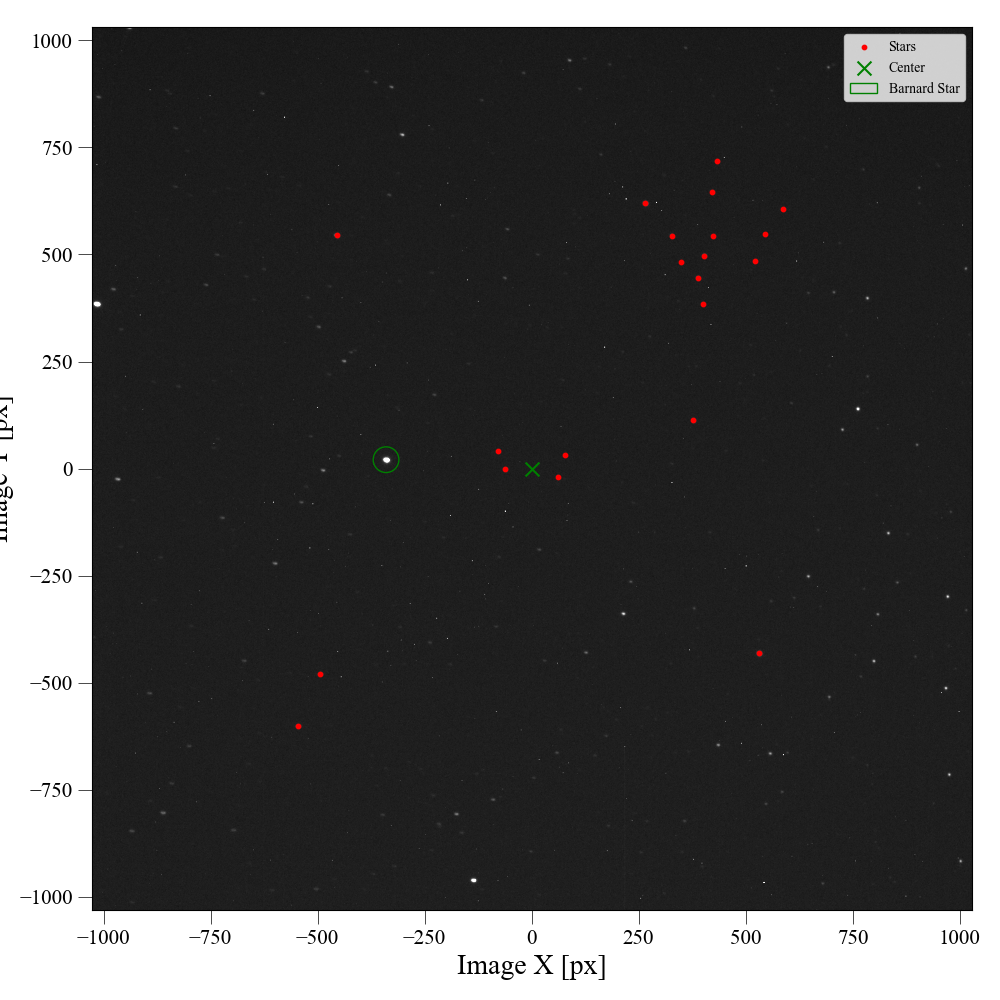
\includegraphics[scale=0.45]{barnard_sky}
                \captionsetup{justification=centering, font=footnotesize}
                \captionof{figure}{Snímek noční oblohy s vyznačenými hvězdami, Barnardovou hvězdou a centrem čipu}
                \label{fig:barnard_sky}
                \vspace{10pt}
                \raggedright 

                \vspace{10pt}   
                \par \centering
                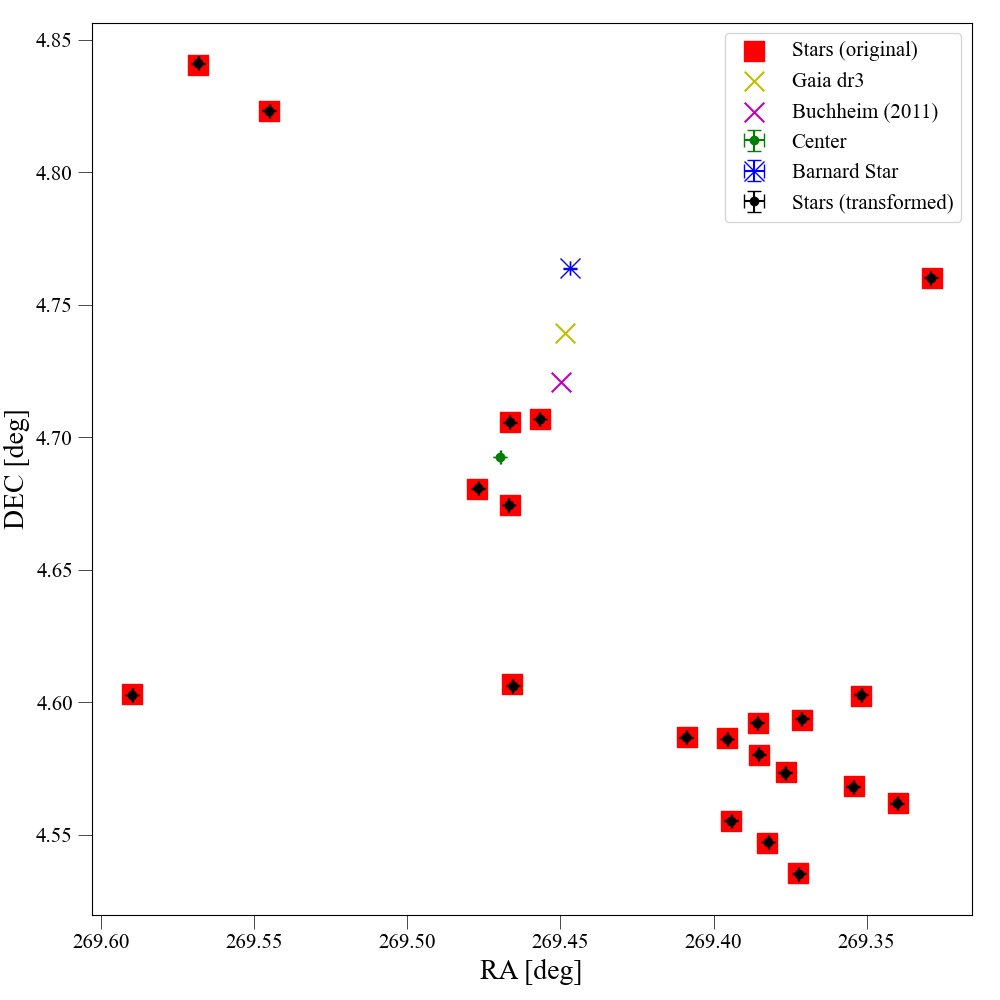
\includegraphics[scale=0.45]{barnard_radec}
                \captionsetup{justification=centering, font=footnotesize}
                \captionof{figure}{Graf Ra a Dec souřadnic hvězd z Aladinu a získaných z obrázku, Barnardova hvězda je vyznačena modřym křížem}
                \label{fig:barnard_radec}
                \vspace{10pt}
                \raggedright 

            \begin{center}
                \subsection{Tabulka 1: Souřadnice hvězd a residua transformace}
                    \pgfplotstabletypeset[
                        col sep=comma, % Defines the separator, comma for CSV
                        string type, % Treats columns as strings (not math mode)
                        every head row/.style={before row=\toprule,after row=\midrule},
                        every last row/.style={after row=\bottomrule},
                    ]{data/positions_with_residuals.csv} 
            \end{center}

\begin{thebibliography}{9}
    \bibitem{github}
        1. Praktikum-z-astronomie, Available online: \url{https://github.com/PoruchikRzhevsky/Praktikum-z-astronomie}
    \bibitem{aladin} 
        2. Aladin Lite, Available online: \url{https://aladin.cds.unistra.fr/AladinLite/}
    \bibitem{Buchheim}
        3. Buchheim, Robert K, 2011, Society for Astronomical Sciences Annual Symposium, 109-114, Available online: \url{https://ui.adsabs.harvard.edu/abs/2011SASS...30..109B}
    \bibitem{Gaia Collaboration}
        4. Gaia Data Release 3. Summary of the content and survey properties, 2023, A\&A, 674, id.A1, 22 pp., Available online: \url{https://ui.adsabs.harvard.edu/abs/2023A%26A...674A...1G}
\end{thebibliography}
\end{document}